%!TEX root=../oi-magistr-si.tex
\section[NUR - Prototypování uživatelských rozhraní]{Prototypování uživatelských rozhraní}
Prototypování se dělá v ranných fázích návrhu. Rozděluje na \textbf{Low-Fidelity} a \textbf{High-Fidelity} prototypování.

\subsection{Low-Fidelity}
První náčrtky rozhraní. Jsou to víceméně narychlo načmárané skicy bez detailů, spiše jde o základní rozvržení (layout) prvků, žádná interakce. Typicky skicy na papíru nebo na elektronických prototypovacích SW (není na finálním zařízení). Je to spíše o rychlém zhodnocení nápadů, které jsou převedeny na papírový prototyp.

\begin{itemize}[itemsep=0px]
\item velké množství nápadů/alternativ
\item krátká doba vývoje - hodiny/dny
\item neběží na finálním zařízení
\item bez interakce
\item testování v laboratoři
\end{itemize}

\vspace{20px}

\begin{figure}[h!]
\centering
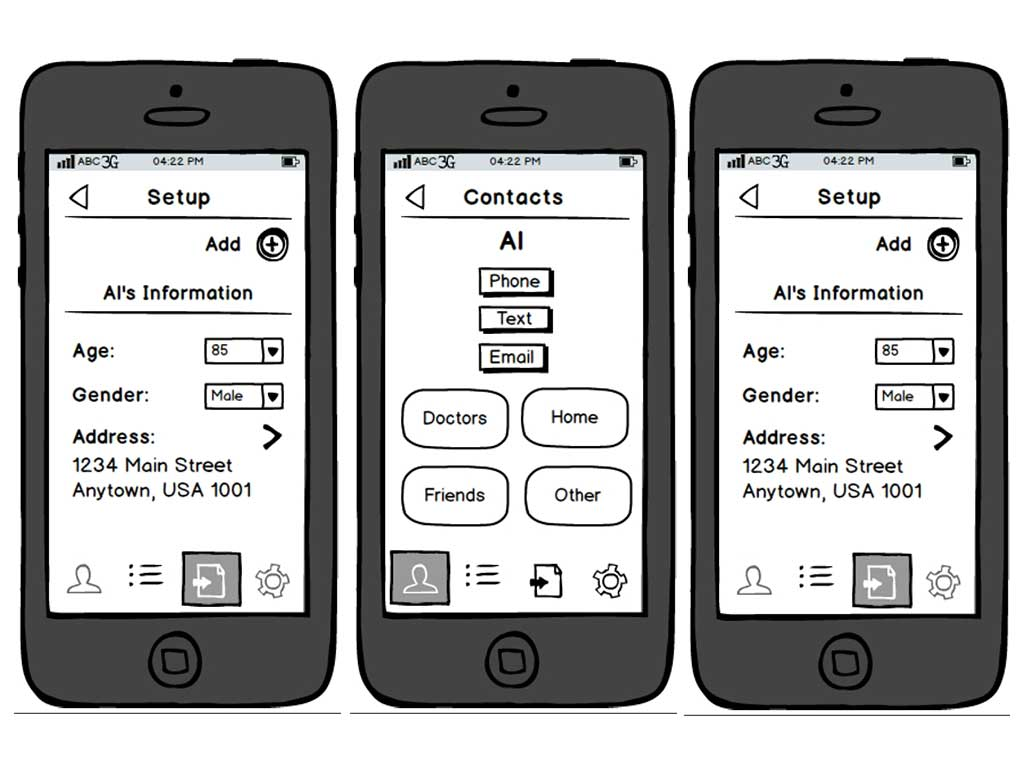
\includegraphics[width=110mm]{06/images/lofi}
\end{figure}

\vspace{20px}

Např. prototypování mobilní app. Vytvoří se několik papírků, každý popisuje krok aplikace. Interakce v podobě fiktvního klikání na papír, dochází k výměně papírků (změna stavu) a tím dochází k fiktivní interakci.

\subsection{High-Fidelity}
Iluze finálního vizuálního (i interagujícího) návrhu. Vzhled by měl následovat \textit{guidelines} cílové platformy (MS Windows, Android, iOS, ..). Prototyp již ve funkční podobě na cílovém zařízení, např. na telefonu. Interakce realizována jakoby to byla již výsledná aplikace, ovšem logika ještě nemusí být implementována (dummy data, \textit{Wizard of Oz}, atd.,). Hlavní části

\begin{itemize}[itemsep=0px]
\item málo alternativ (pokud vůbec nějaké jsou)
\item dlouhá doba vývoje - dny/týdny
\item dostupné na finálním zařízení
\item podoba a interakce téměr podobná té finální
\item testování v laboratoři a v \uv{terénu} (v reálných podmínkách využití)
\end{itemize}

\begin{figure}[h!]
\centering
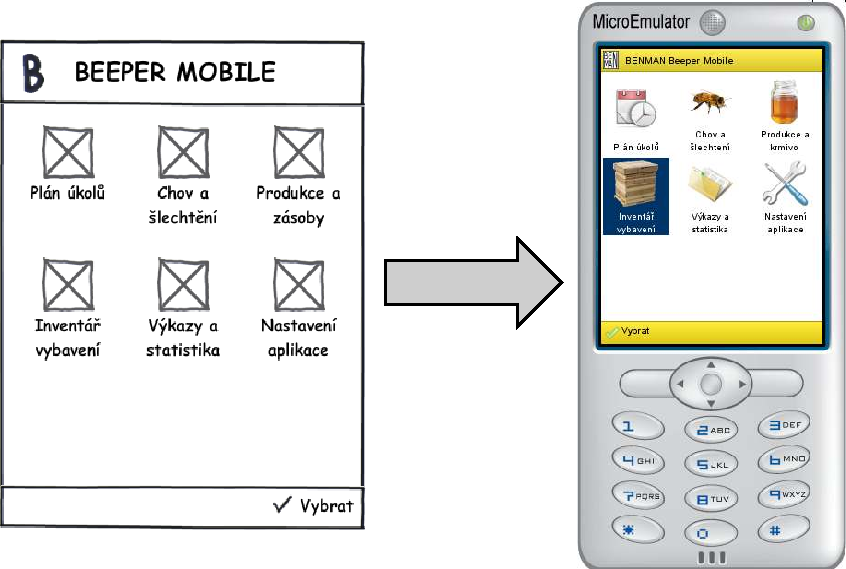
\includegraphics[width=80mm]{06/images/hifi}
\end{figure}

\paragraph{Problémy s prototypováním}
\begin{itemize}[itemsep=0px]
\item U lo-fi prototypů dochází ke skipování hlubokých (detailních) uživatelských požadavků
\item user confusion: hi-fi prototyp vs. finální aplikace
\item drahé a žrout času (speciálně hi-fi)
\end{itemize}